\documentclass[10pt]{article}

\usepackage{amsmath,amscd}
\usepackage{amssymb,array}
\usepackage{amsfonts,latexsym}
\usepackage[mathscr]{euscript}
\usepackage{graphicx,subfig,wrapfig}
\usepackage{times}
\usepackage{psfrag,epsfig}
\usepackage{verbatim}
\usepackage{tabularx}
\usepackage[toc,page]{appendix}

\newcommand{\matlab}[1]{\texttt{#1}}
\newcommand{\setname}[1]{\textsl{#1}}
\newcommand{\Ce}{\mathbb{C}}
\newcommand{\Ree}{\mathbb{R}}
\newcommand{\p}{\begin{pmatrix}}
\newcommand{\pp}{\end{pmatrix}}
\newcommand{\bm}{\begin{bmatrix}}
\newcommand{\bb}{\end{bmatrix}}
\newcommand{\eul}[1]{e^{#1}}

\begin{document}

\title{ \vspace{-30mm}Systems Bioengineering 3\\Homework 12}
\author{Greg Kiar}

\maketitle
\begin{enumerate}
\item
%q1
\begin{enumerate}
\item For the following evaluation of average time, we make use of the fact that the transcript follows an exponential trend.
\begin{align*}
E(T) = t_{avg} &= \int_0^{\infty} t e^{-\alpha t} dt \\
&= \alpha \begin{bmatrix} \frac{-t}{\alpha} - \int_0^{\infty} \frac{1}{\alpha} e^{-\alpha t} dt \end{bmatrix} \\
&= \alpha \begin{bmatrix} \frac{-t}{\alpha}e^{-\alpha t} + \frac{-1}{\alpha^2} e^{-\alpha t}\end{bmatrix}_{0,t} \\
t_{avg} &= \frac{1}{\alpha} = 10 \text{min}
\end{align*}
At equilibrium, $\beta = \alpha n$, $\therefore \mu_n = 10$ at equilibrium. The variance is $10$ since for independent stochastic events $\sigma_n^2 = \mu_n$.
\item We can see that the ODE of this system is: $\dot{X}(t) = \beta - \alpha X(t)$. Solving this model using the equation: \begin{align*} \dot{X} &= \frac{d}{dX} ln(X(t)) \\ 0 &= \frac{d}{dX}\begin{pmatrix} ln(\frac{\beta}{\alpha} - n) \end{pmatrix} \\
n &= \frac{\beta}{\alpha} = 10 \end{align*}
\item Source code for this part was provided by the TAs. It has been modified slightly and is attached in an appendix.
\item When starting the simulation at $n=10$ and running it for $10,000$ min, the mean and variance were $\mu = 10.1287$ and $\sigma^2 = 9.8604$, respectively. These values are near but not exactly expected values. This makes sense because the discrete stochastic system has a finitely small timestep. If the timesteps were infinitely small or the trial infinitely long, the values would approach the theoretical values.
\end{enumerate}

\item \begin{enumerate}
\item Solving $\dot{X}(t) = \beta - \alpha X(t)$ for the case prior to equilibrium allows us to use the Laplace transform. The solution of this system becomes \begin{align*} X(t) = \frac{\beta}{\alpha} (1 - e^{-\alpha t}) \end{align*}
\item Shown below is the solution for $1000$ randomly generated trajectories each for $100 min$. \\ 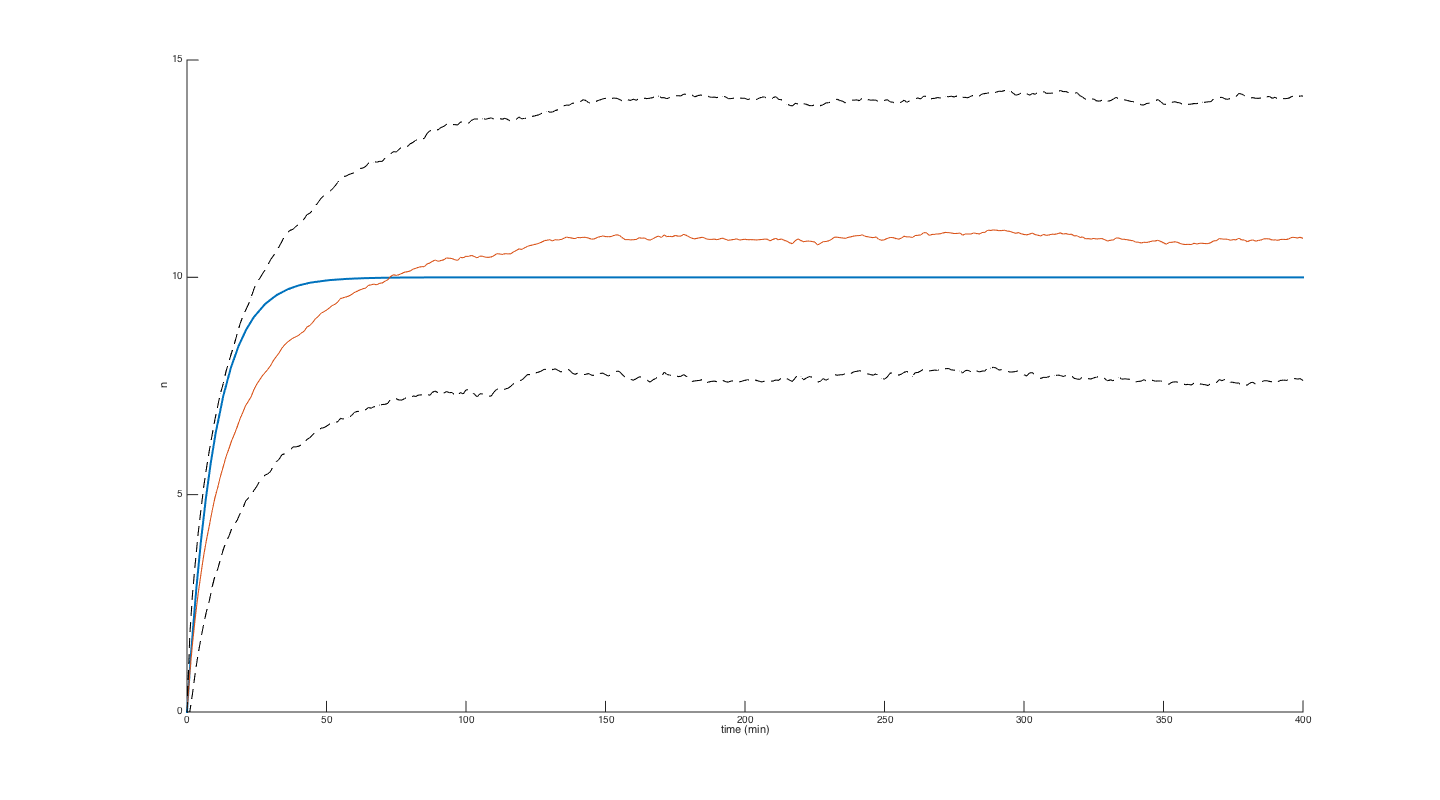
\includegraphics[scale=0.2]{sbe3hw12q2b.png}
\item It can be seen by the figure below, a plot of the variance, that the variance follows the same exponential trend as the random variable $n$. From this, we can set an approximate equation for the variance to be $\sigma^2 = \frac{\beta}{\alpha} (1 - e^{-\alpha t}) $. From this we can see that the variance is at a maximum as $t \to \infty$. 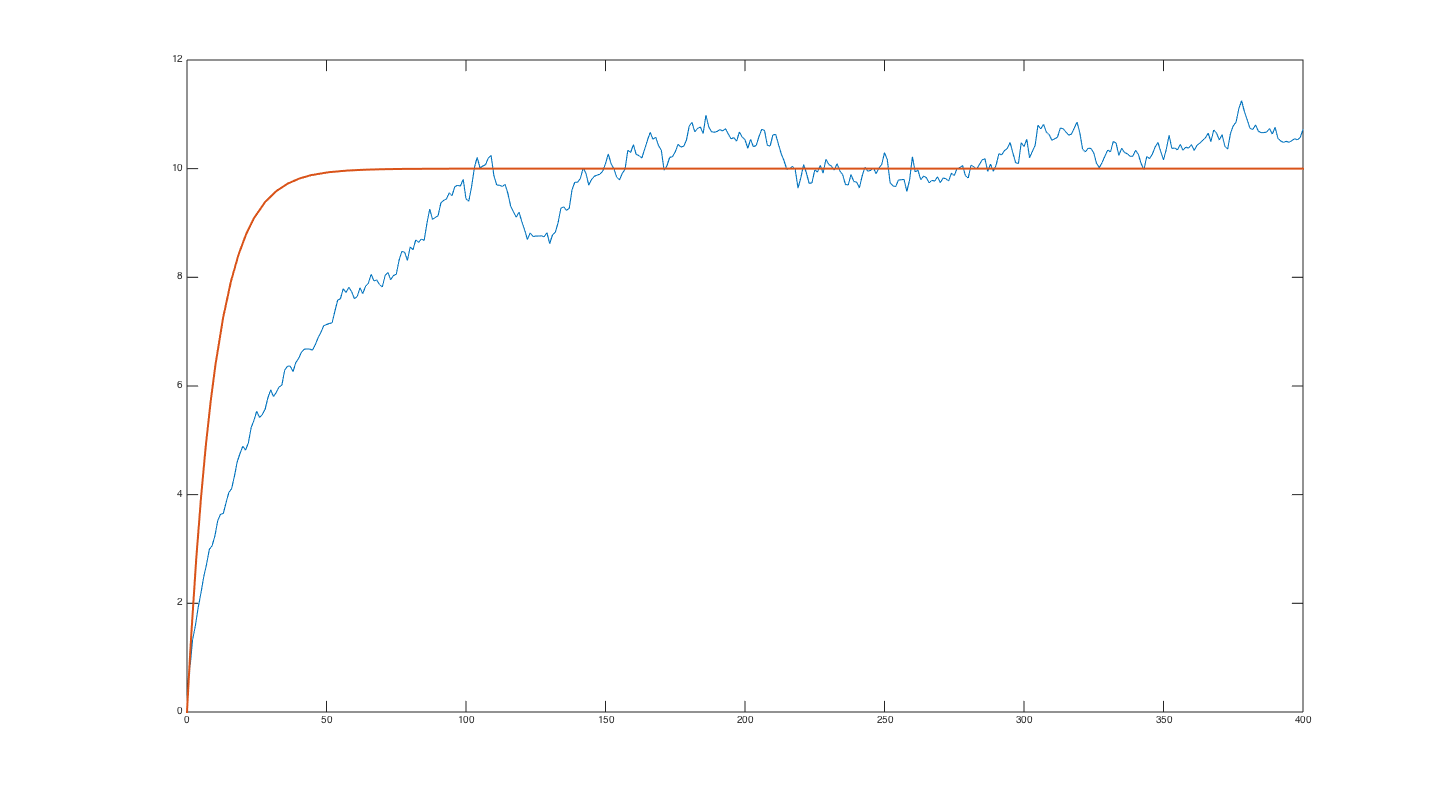
\includegraphics[scale=0.2]{sbe3hw12q2c.png}
\end{enumerate}

\item \begin{enumerate}
\item Similarly to the equation found in 2a), we can solve $ \dot{X}(t) = \frac{\beta}{b} - \alpha X(t) $, where $b=5$ here. The result for $X(t)$ is as follows: \begin{align*} X(t) &= \frac{\beta}{b \alpha} (1 - e^{-\alpha t})\end{align*}
We can see from this result that the burst size, $b$, affects the forward rate of the system. The forward rate$ = \frac{\beta}{b}$.
\item Simulating the stochastic and ODE models of this system for $10,000 min$ with the inital condition $X(0) = n(0) = 2$, the equilibrium value, the discrete model produced the values shown below. \begin{align*} \text{Discrete} && \mu &= 12.0428 && \sigma^2 = 30.3180 \\ \end{align*}
\item For the stochastic system with larger burst sizes, the mean and variance both increase. When testing this for different burst sizes, an approximately linear relationship is observed for both the mean and variance values. This relationship does not change as $\beta$ or $\alpha$ increase and decrease simultaneously to one another. The approximate expressions are as follows: \begin{align*} \mu &= \frac{\beta}{\alpha}\\ \sigma^2 &= \frac{2 \beta}{b \alpha} \end{align*}
\end{enumerate}
\end{enumerate}
\newpage
\begin{appendices}
\section{Trajectories}

% This LaTeX was auto-generated from MATLAB code.
% To make changes, update the MATLAB code and republish this document.

\documentclass{article}
\usepackage{graphicx}
\usepackage{color}

\sloppy
\definecolor{lightgray}{gray}{0.5}
\setlength{\parindent}{0pt}

\begin{document}

    
    \begin{verbatim}
function [T, N] = get_trajectory(n_0, t_max, burst)
% GET_TRAJECTORY - Computes a single Gillespie trajectory.
% Outputs:
% T - transition times
% N - counts at each transition time
% Inputs:
% n_0 - initial number of molecules.
% t_max - length of time of the simulation.

global a b
t = 0;
j = 1;
T(1) = 0;
N(1) = n_0;
while t < t_max
    j = j+1;
    dt = exprnd(b + a*N(j-1));
    t = t + dt;
    T(j) = t;
    if rand < b/(b+a*N(j-1))
        N(j) = N(j-1) + burst;
    else
        N(j) = N(j-1) - 1;
        if N(j) <= 0
            N(j) = 0;
        end
    end

end
end
\end{verbatim}

        \color{lightgray} \begin{verbatim}Error using get_trajectory (line 14)
Not enough input arguments.
\end{verbatim} \color{black}
    


\end{document}
    

\section{Example main script}
\input{Prob2_forStudents}
\end{appendices}
\end{document}
